\documentclass[11pt,a4paper]{article}
\usepackage[utf8]{inputenc}
\usepackage[T1]{fontenc}
\usepackage{amsmath,amssymb,amsfonts}
\usepackage[margin=1in]{geometry}
\usepackage{enumitem}
\usepackage{hyperref}
\usepackage{fancyhdr}
\usepackage{titlesec}
\usepackage{tocloft}
\usepackage{tikz}
\usepackage{pgfplots}
\pgfplotsset{compat=1.17}
\usetikzlibrary{patterns,arrows.meta,calc,decorations.markings,shapes.geometric}
\newtheorem{example}{Example}
\newtheorem{theorem}{Theorem}
\newtheorem{definition}{Definition}
\newtheorem{lemma}{Lemma}
\newtheorem{corollary}{Corollary}
\newtheorem{remark}{Remark}
\pagestyle{fancy}
\fancyhf{}
\fancyhead[L]{\small Lecture Notes: Complex Numbers and Polar Coordinates}
\fancyhead[R]{\small \thepage}
\renewcommand{\headrulewidth}{0.4pt}
\titleformat{\section}{\Large\bfseries}{Section \thesection}{1em}{}
\titleformat{\subsection}{\large\bfseries}{\thesubsection}{1em}{}
\renewcommand{\cftsecfont}{\bfseries}
\renewcommand{\cftsubsecfont}{\normalfont}
\begin{document}
\begin{titlepage}
\centering
\vspace*{4cm}
{\Huge\bfseries Lecture Notes:\\ Complex Numbers and Polar Coordinates\par}
\vspace{1cm}
{\Large Calculus I\par}
\vspace{2cm}
{\large \textbf{Author:} Bakdaulet Sotsial\par}
\vspace{1cm}
\vfill
{\small Astana IT University \par}
\vspace*{2cm}
\end{titlepage}
\tableofcontents
\newpage
\section{Complex Numbers}
\begin{definition}[Imaginary Unit]
The \textit{imaginary unit}, denoted by $i$, is defined by the property
\[
i^2 = -1.
\]
Equivalently, $i = \sqrt{-1}$.
\end{definition}
\begin{definition}[Complex Number]
A \textit{complex number} is a number of the form
\[
z = a + bi,
\]
where $a$ and $b$ are real numbers. The real number $a$ is called the \textit{real part} of $z$, denoted $\operatorname{Re}(z) = a$. The real number $b$ is called the \textit{imaginary part} of $z$, denoted $\operatorname{Im}(z) = b$. The set of all complex numbers is denoted by $\mathbb{C}$.
\end{definition}
\begin{remark}
If $b = 0$, then $z = a$ is a real number, so $\mathbb{R} \subset \mathbb{C}$. If $a = 0$ and $b \neq 0$, then $z = bi$ is called a \textit{pure imaginary number}.
\end{remark}
\begin{example}
The following are complex numbers:
\begin{enumerate}
\item $z = 3 + 4i$, with $\operatorname{Re}(z) = 3$ and $\operatorname{Im}(z) = 4$.
\item $z = -2 - i$, with $\operatorname{Re}(z) = -2$ and $\operatorname{Im}(z) = -1$.
\item $z = 5$, with $\operatorname{Re}(z) = 5$ and $\operatorname{Im}(z) = 0$.
\item $z = 7i$, with $\operatorname{Re}(z) = 0$ and $\operatorname{Im}(z) = 7$.
\end{enumerate}
\end{example}
\begin{definition}[Equality of Complex Numbers]
Two complex numbers $z_1 = a_1 + b_1 i$ and $z_2 = a_2 + b_2 i$ are equal if and only if $a_1 = a_2$ and $b_1 = b_2$.
\end{definition}
\begin{definition}[Complex Conjugate]
The \textit{complex conjugate} of $z = a + bi$, denoted $\bar{z}$, is defined by
\[
\bar{z} = a - bi.
\]
\end{definition}
\begin{definition}[Modulus]
The \textit{modulus} (or absolute value) of $z = a + bi$, denoted $|z|$, is defined by
\[
|z| = \sqrt{a^2 + b^2}.
\]
\end{definition}
\begin{theorem}[Properties of the Conjugate and Modulus]
For any complex numbers $z, z_1, z_2 \in \mathbb{C}$:
\begin{enumerate}
\item $\overline{z_1 + z_2} = \bar{z_1} + \bar{z_2}$.
\item $\overline{z_1 z_2} = \bar{z_1} \cdot \bar{z_2}$.
\item $z \bar{z} = |z|^2$.
\item $|z_1 z_2| = |z_1| |z_2|$.
\item $\left| \frac{z_1}{z_2} \right| = \frac{|z_1|}{|z_2|}$, provided $z_2 \neq 0$.
\item $|z_1 + z_2| \leq |z_1| + |z_2|$ (Triangle Inequality).
\end{enumerate}
\end{theorem}
\begin{proof}
For (3): If $z = a + bi$, then $z\bar{z} = (a+bi)(a-bi) = a^2 - (bi)^2 = a^2 + b^2 = |z|^2$. The other properties follow by direct computation.
\end{proof}
\section{Operations with Complex Numbers}
\begin{definition}[Addition and Subtraction]
If $z_1 = a_1 + b_1 i$ and $z_2 = a_2 + b_2 i$, then
\[
z_1 + z_2 = (a_1 + a_2) + (b_1 + b_2) i,
\]
\[
z_1 - z_2 = (a_1 - a_2) + (b_1 - b_2) i.
\]
\end{definition}
\begin{definition}[Multiplication]
If $z_1 = a_1 + b_1 i$ and $z_2 = a_2 + b_2 i$, then
\[
z_1 z_2 = (a_1 + b_1 i)(a_2 + b_2 i) = (a_1 a_2 - b_1 b_2) + (a_1 b_2 + a_2 b_1) i.
\]
\end{definition}
\begin{definition}[Division]
If $z_1 = a_1 + b_1 i$ and $z_2 = a_2 + b_2 i \neq 0$, then
\[
\frac{z_1}{z_2} = \frac{z_1 \bar{z_2}}{z_2 \bar{z_2}} = \frac{(a_1 + b_1 i)(a_2 - b_2 i)}{a_2^2 + b_2^2} = \frac{a_1 a_2 + b_1 b_2}{a_2^2 + b_2^2} + \frac{a_2 b_1 - a_1 b_2}{a_2^2 + b_2^2} i.
\]
\end{definition}
\begin{example}
Given $z_1 = 3 + 4i$ and $z_2 = 1 - 2i$, compute $z_1 + z_2$, $z_1 - z_2$, $z_1 z_2$, and $\frac{z_1}{z_2}$.
\[
z_1 + z_2 = (3+1) + (4-2)i = 4 + 2i.
\]
\[
z_1 - z_2 = (3-1) + (4+2)i = 2 + 6i.
\]
\[
z_1 z_2 = (3)(1) - (4)(-2) + [(3)(-2) + (1)(4)]i = 3 + 8 + (-6 + 4)i = 11 - 2i.
\]
\[
\frac{z_1}{z_2} = \frac{(3+4i)(1+2i)}{(1-2i)(1+2i)} = \frac{3 + 6i + 4i + 8i^2}{1 + 4} = \frac{-5 + 10i}{5} = -1 + 2i.
\]
\end{example}
\begin{example}
Compute $i^n$ for various integers $n$.
\[
i^1 = i, \quad i^2 = -1, \quad i^3 = -i, \quad i^4 = 1, \quad i^5 = i, \dots
\]
The powers of $i$ cycle with period 4: $i, -1, -i, 1$.
\end{example}
\begin{theorem}[Geometric Interpretation]
A complex number $z = a + bi$ can be represented as the point $(a, b)$ in the \textit{complex plane} (or Argand diagram), where the horizontal axis is the real axis and the vertical axis is the imaginary axis. The modulus $|z|$ is the distance from the origin to the point $(a, b)$, and the conjugate $\bar{z}$ is the reflection across the real axis.
\end{theorem}
\begin{center}
\begin{tikzpicture}[scale=1.1]
\draw[->] (-3,0) -- (3.5,0) node[right] {$\operatorname{Re}$};
\draw[->] (0,-3) -- (0,3.2) node[above] {$\operatorname{Im}$};
\draw[gray, dashed] (2,1.5) -- (2,0);
\draw[gray, dashed] (2,1.5) -- (0,1.5);
\filldraw[blue] (2,1.5) circle (2pt);
\node[blue, above right] at (2,1.5) {$z = a+bi$};
\draw[blue, thick, ->] (0,0) -- (2,1.5);
\filldraw[red] (2,-1.5) circle (2pt);
\node[red, below right] at (2,-1.5) {$\bar{z} = a-bi$};
\draw[red, thick, ->] (0,0) -- (2,-1.5);
\draw[gray, dashed] (2,1.5) -- (2,-1.5);
\node at (1.0,0.9) {$|z|$};
\node at (2.6,0) {$a$};
\node at (0.3,1.5) {$b$};
\node at (0.3,-1.5) {$-b$};
\end{tikzpicture}
\end{center}
\section{Polar Coordinates}
\begin{definition}[Polar Coordinate System]
The \textit{polar coordinate system} represents points in the plane using an ordered pair $(r, \theta)$, where $r$ is the directed distance from the origin (called the \textit{pole}), and $\theta$ is the angle measured counterclockwise from the positive $x$-axis (called the \textit{polar axis}).
\end{definition}
\begin{theorem}[Conversion Between Cartesian and Polar Coordinates]
Given Cartesian coordinates $(x, y)$ and polar coordinates $(r, \theta)$:
\[
x = r \cos \theta, \quad y = r \sin \theta,
\]
\[
r^2 = x^2 + y^2, \quad \tan \theta = \frac{y}{x} \quad (x \neq 0).
\]
\end{theorem}
\begin{proof}
These follow directly from the definitions of sine and cosine in a right triangle with hypotenuse $r$ and the Pythagorean theorem.
\end{proof}
\begin{center}
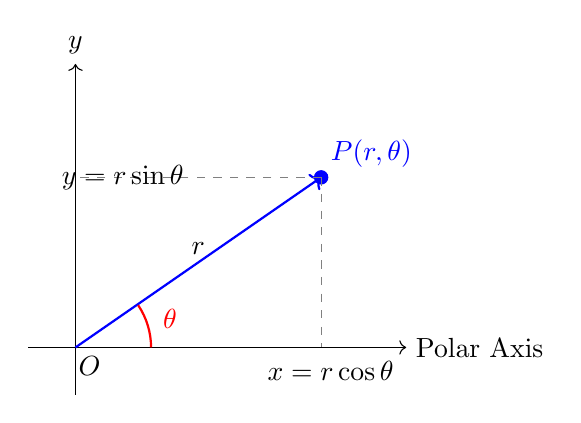
\begin{tikzpicture}[scale=1.2]
\draw[->] (-0.5,0) -- (3.5,0) node[right] {Polar Axis};
\draw[->] (0,-0.5) -- (0,3.0) node[above] {$y$};
\filldraw[blue] (2.6,1.8) circle (2pt);
\node[blue, above right] at (2.6,1.8) {$P(r, \theta)$};
\draw[blue, thick, ->] (0,0) -- (2.6,1.8);
\draw[gray, dashed] (2.6,1.8) -- (2.6,0);
\draw[gray, dashed] (2.6,1.8) -- (0,1.8);
\draw[red, thick] (0.8,0) arc (0:34:0.8);
\node[red] at (1.0,0.3) {$\theta$};
\node at (1.3,1.05) {$r$};
\node at (2.7,-0.25) {$x = r\cos\theta$};
\node at (0.5,1.8) {$y = r\sin\theta$};
\node at (0.15,-0.2) {$O$};
\end{tikzpicture}
\end{center}
\begin{example}
Convert the polar point $\left( 2, \frac{\pi}{6} \right)$ to Cartesian coordinates.
\[
x = 2 \cos \frac{\pi}{6} = 2 \cdot \frac{\sqrt{3}}{2} = \sqrt{3}, \quad y = 2 \sin \frac{\pi}{6} = 2 \cdot \frac{1}{2} = 1.
\]
Thus, the Cartesian coordinates are $(\sqrt{3}, 1)$.
\end{example}
\begin{example}
Convert the Cartesian point $(-1, 1)$ to polar coordinates.
\[
r = \sqrt{(-1)^2 + 1^2} = \sqrt{2}.
\]
Since the point is in the second quadrant, $\theta = \frac{3\pi}{4}$. Thus, $(\sqrt{2}, \frac{3\pi}{4})$.
\end{example}
\begin{remark}[Non-Uniqueness of Polar Coordinates]
A point in the plane can be represented by infinitely many polar coordinate pairs. If $(r, \theta)$ represents a point, then so do $(r, \theta + 2n\pi)$ for any integer $n$, and $(-r, \theta + (2n+1)\pi)$ for any integer $n$.
\end{remark}
\section{Graphing Polar Coordinate Equations}
\begin{definition}[Polar Curve]
The graph of a polar equation $r = f(\theta)$ consists of all points $P$ that have at least one polar representation $(r, \theta)$ satisfying the equation.
\end{definition}
\begin{theorem}[Symmetry Tests for Polar Graphs]
\begin{enumerate}
\item \textbf{Symmetry about the polar axis ($x$-axis):} The graph is symmetric if replacing $(r, \theta)$ with $(r, -\theta)$ or $(-r, \pi - \theta)$ yields an equivalent equation.
\item \textbf{Symmetry about the line $\theta = \frac{\pi}{2}$ ($y$-axis):} The graph is symmetric if replacing $(r, \theta)$ with $(r, \pi - \theta)$ or $(-r, -\theta)$ yields an equivalent equation.
\item \textbf{Symmetry about the pole (origin):} The graph is symmetric if replacing $(r, \theta)$ with $(-r, \theta)$ or $(r, \theta + \pi)$ yields an equivalent equation.
\end{enumerate}
\end{theorem}
\begin{example}[Circle]
Sketch the graph of $r = 3$.
This equation describes all points at a distance 3 from the pole. The graph is a circle of radius 3 centered at the origin.
\begin{center}
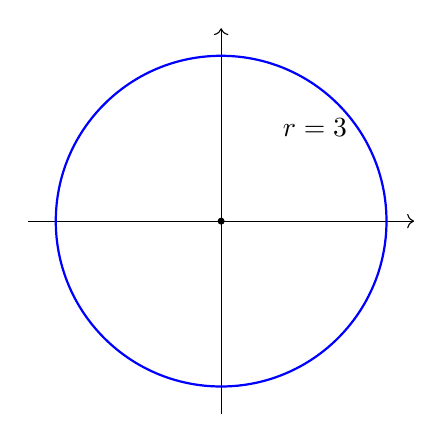
\begin{tikzpicture}[scale=0.7]
\draw[->] (-3.5,0) -- (3.5,0);
\draw[->] (0,-3.5) -- (0,3.5);
\draw[blue, thick] (0,0) circle (3);
\filldraw (0,0) circle (1.5pt);
\node at (1.7,1.7) {$r=3$};
\end{tikzpicture}
\end{center}
\end{example}
\begin{example}[Cardioid]
Sketch the graph of $r = 1 + \cos \theta$.
This is a cardioid. Compute values: at $\theta = 0$, $r = 2$; at $\theta = \frac{\pi}{2}$, $r = 1$; at $\theta = \pi$, $r = 0$; at $\theta = \frac{3\pi}{2}$, $r = 1$. The graph is symmetric about the polar axis.
\begin{center}
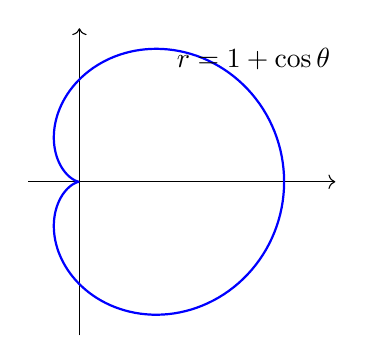
\begin{tikzpicture}[scale=1.3]
\draw[->] (-0.5,0) -- (2.5,0);
\draw[->] (0,-1.5) -- (0,1.5);
\draw[blue, thick, domain=0:360, samples=200] plot ({(1+cos(\x))*cos(\x)}, {(1+cos(\x))*sin(\x)});
\node at (1.7,1.2) {$r=1+\cos\theta$};
\end{tikzpicture}
\end{center}
\end{example}
\begin{example}[Rose Curve]
Sketch the graph of $r = \cos 2\theta$.
This is a four-petaled rose. At $\theta = 0$, $r = 1$; at $\theta = \frac{\pi}{4}$, $r = 0$; at $\theta = \frac{\pi}{2}$, $r = -1$; and so on. The curve has four petals.
\begin{center}
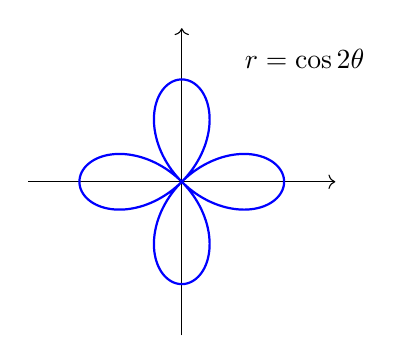
\begin{tikzpicture}[scale=1.3]
\draw[->] (-1.5,0) -- (1.5,0);
\draw[->] (0,-1.5) -- (0,1.5);
\draw[blue, thick, domain=0:360, samples=300] plot ({cos(2*\x)*cos(\x)}, {cos(2*\x)*sin(\x)});
\node at (1.2,1.2) {$r=\cos 2\theta$};
\end{tikzpicture}
\end{center}
\end{example}
\begin{example}[Lemniscate]
Sketch the graph of $r^2 = 4 \cos 2\theta$.
This is a lemniscate (figure-eight shape). The curve is defined only when $\cos 2\theta \geq 0$, i.e., $\theta \in [-\frac{\pi}{4}, \frac{\pi}{4}] \cup [\frac{3\pi}{4}, \frac{5\pi}{4}]$.
\begin{center}
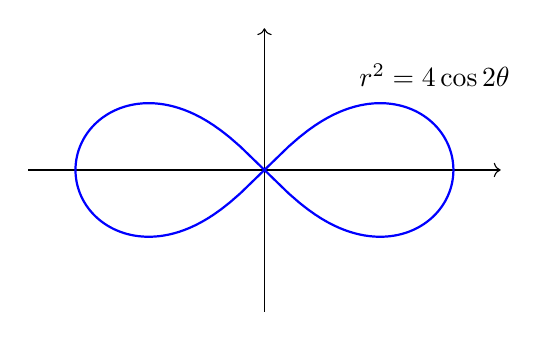
\begin{tikzpicture}[scale=1.2]
\draw[->] (-2.5,0) -- (2.5,0);
\draw[->] (0,-1.5) -- (0,1.5);
\draw[blue, thick, domain=-45:45, samples=100] plot ({2*sqrt(cos(2*\x))*cos(\x)}, {2*sqrt(cos(2*\x))*sin(\x)});
\draw[blue, thick, domain=135:225, samples=100] plot ({2*sqrt(cos(2*\x))*cos(\x)}, {2*sqrt(cos(2*\x))*sin(\x)});
\node at (1.8,1.0) {$r^2=4\cos 2\theta$};
\end{tikzpicture}
\end{center}
\end{example}
\begin{theorem}[Common Polar Curves]
\begin{itemize}
\item \textbf{Circle:} $r = a$, or $r = 2a \cos \theta$, or $r = 2a \sin \theta$.
\item \textbf{Cardioid:} $r = a \pm a \cos \theta$ or $r = a \pm a \sin \theta$.
\item \textbf{Limaçon:} $r = a \pm b \cos \theta$ or $r = a \pm b \sin \theta$.
\item \textbf{Rose:} $r = a \cos n\theta$ or $r = a \sin n\theta$ (has $n$ petals if $n$ is odd, $2n$ petals if $n$ is even).
\item \textbf{Lemniscate:} $r^2 = a^2 \cos 2\theta$ or $r^2 = a^2 \sin 2\theta$.
\item \textbf{Spiral:} $r = a\theta$ (Archimedean) or $r = a e^{b\theta}$ (logarithmic).
\end{itemize}
\end{theorem}
\section{Integration in Polar Coordinates}
\begin{definition}[Area Element in Polar Coordinates]
A small sector of a polar curve with angle $d\theta$ and radius $r$ has area approximately $\frac{1}{2} r^2 \, d\theta$. This is the basis for integration in polar coordinates.
\end{definition}
\begin{theorem}[Area in Polar Coordinates]
If $f$ is continuous and non-negative on the interval $[\alpha, \beta]$, then the area $A$ of the region bounded by the graph of $r = f(\theta)$ and the rays $\theta = \alpha$ and $\theta = \beta$ is
\[
A = \int_{\alpha}^{\beta} \frac{1}{2} [f(\theta)]^2 \, d\theta = \int_{\alpha}^{\beta} \frac{1}{2} r^2 \, d\theta.
\]
\end{theorem}
\begin{proof}
Divide $[\alpha, \beta]$ into $n$ subintervals with angles $\theta_i$. In each subinterval, choose a sample angle $\theta_i^*$ and approximate the area by a circular sector with radius $f(\theta_i^*)$ and central angle $\Delta \theta$. The area of the sector is $\frac{1}{2} [f(\theta_i^*)]^2 \Delta \theta$. Summing and taking the limit as $n \to \infty$ gives the integral.
\end{proof}
\begin{center}
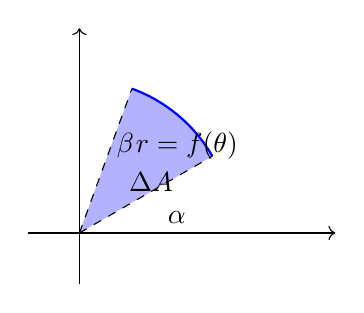
\begin{tikzpicture}[scale=1.3]
\draw[->] (-0.5,0) -- (2.5,0);
\draw[->] (0,-0.5) -- (0,2.0);
\fill[blue!30] (0,0) -- (30:1.5) arc (30:70:1.5) -- cycle;
\draw[blue, thick] (30:1.5) arc (30:70:1.5);
\node at (0.7,0.5) {$\Delta A$};
\draw[dashed] (0,0) -- (30:1.5);
\draw[dashed] (0,0) -- (70:1.5);
\node at (0.95,0.15) {$\alpha$};
\node at (0.45,0.85) {$\beta$};
\node at (1.05,0.85) {$r=f(\theta)$};
\end{tikzpicture}
\end{center}
\begin{example}
Find the area enclosed by the cardioid $r = 1 + \cos \theta$.
The curve is traced completely as $\theta$ goes from $0$ to $2\pi$.
\[
A = \int_0^{2\pi} \frac{1}{2} (1 + \cos \theta)^2 \, d\theta = \frac{1}{2} \int_0^{2\pi} (1 + 2\cos \theta + \cos^2 \theta) \, d\theta.
\]
Using $\cos^2 \theta = \frac{1 + \cos 2\theta}{2}$,
\[
A = \frac{1}{2} \int_0^{2\pi} \left( 1 + 2\cos \theta + \frac{1 + \cos 2\theta}{2} \right) d\theta = \frac{1}{2} \int_0^{2\pi} \left( \frac{3}{2} + 2\cos \theta + \frac{1}{2}\cos 2\theta \right) d\theta.
\]
\[
A = \frac{1}{2} \left[ \frac{3\theta}{2} + 2\sin \theta + \frac{\sin 2\theta}{4} \right]_0^{2\pi} = \frac{1}{2} \cdot 3\pi = \frac{3\pi}{2}.
\]
\end{example}
\begin{example}
Find the area of one petal of the rose $r = \cos 2\theta$.
One petal is traced as $\theta$ goes from $-\frac{\pi}{4}$ to $\frac{\pi}{4}$.
\[
A = \int_{-\pi/4}^{\pi/4} \frac{1}{2} \cos^2 2\theta \, d\theta = \frac{1}{2} \int_{-\pi/4}^{\pi/4} \frac{1 + \cos 4\theta}{2} \, d\theta = \frac{1}{4} \left[ \theta + \frac{\sin 4\theta}{4} \right]_{-\pi/4}^{\pi/4}.
\]
\[
A = \frac{1}{4} \left[ \left( \frac{\pi}{4} + 0 \right) - \left( -\frac{\pi}{4} + 0 \right) \right] = \frac{1}{4} \cdot \frac{\pi}{2} = \frac{\pi}{8}.
\]
\end{example}
\begin{theorem}[Area Between Two Polar Curves]
If $r_1 = f(\theta)$ and $r_2 = g(\theta)$ are continuous with $f(\theta) \geq g(\theta) \geq 0$ on $[\alpha, \beta]$, then the area of the region between them is
\[
A = \int_{\alpha}^{\beta} \frac{1}{2} \left( [f(\theta)]^2 - [g(\theta)]^2 \right) d\theta.
\]
\end{theorem}
\begin{example}
Find the area inside $r = 2$ and outside $r = 1 + \cos \theta$.
Intersection: $2 = 1 + \cos \theta \implies \cos \theta = 1 \implies \theta = 0$, but we need the region where $2 \geq 1 + \cos \theta$, i.e., $\cos \theta \leq 1$, which is true except at $\theta = 0$. The full area is
\[
A = \int_0^{2\pi} \frac{1}{2} (4 - (1 + \cos \theta)^2) \, d\theta.
\]
Since $(1 + \cos \theta)^2 = 1 + 2\cos \theta + \cos^2 \theta$, we get
\[
A = \frac{1}{2} \int_0^{2\pi} (3 - 2\cos \theta - \cos^2 \theta) \, d\theta = \frac{1}{2} \int_0^{2\pi} \left( 3 - 2\cos \theta - \frac{1 + \cos 2\theta}{2} \right) d\theta.
\]
\[
A = \frac{1}{2} \int_0^{2\pi} \left( \frac{5}{2} - 2\cos \theta - \frac{\cos 2\theta}{2} \right) d\theta = \frac{1}{2} \left[ \frac{5\theta}{2} - 2\sin \theta - \frac{\sin 2\theta}{4} \right]_0^{2\pi} = \frac{1}{2} \cdot 5\pi = \frac{5\pi}{2}.
\]
\end{example}
\section{Arc Length in Polar Coordinates}
\begin{theorem}[Arc Length in Polar Coordinates]
If $f$ has a continuous derivative on $[\alpha, \beta]$, then the length $L$ of the polar curve $r = f(\theta)$ from $\theta = \alpha$ to $\theta = \beta$ is
\[
L = \int_{\alpha}^{\beta} \sqrt{[f(\theta)]^2 + [f'(\theta)]^2} \, d\theta = \int_{\alpha}^{\beta} \sqrt{r^2 + \left( \frac{dr}{d\theta} \right)^2} \, d\theta.
\]
\end{theorem}
\begin{proof}
Parametrize the polar curve as $x = r \cos \theta = f(\theta) \cos \theta$ and $y = r \sin \theta = f(\theta) \sin \theta$. Then
\[
\frac{dx}{d\theta} = f'(\theta) \cos \theta - f(\theta) \sin \theta, \quad \frac{dy}{d\theta} = f'(\theta) \sin \theta + f(\theta) \cos \theta.
\]
Thus,
\[
\left( \frac{dx}{d\theta} \right)^2 + \left( \frac{dy}{d\theta} \right)^2 = [f'(\theta)]^2 + [f(\theta)]^2 = r^2 + \left( \frac{dr}{d\theta} \right)^2.
\]
The arc length formula for parametric curves gives the result.
\end{proof}
\begin{center}
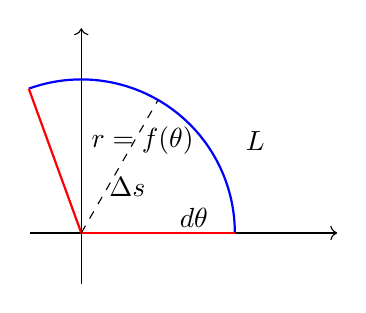
\begin{tikzpicture}[scale=1.3]
\draw[->] (-0.5,0) -- (2.5,0);
\draw[->] (0,-0.5) -- (0,2.0);
\draw[blue, thick, domain=0:110, samples=100] plot ({1.5*cos(\x)}, {1.5*sin(\x)});
\draw[red, thick] (0,0) -- (0:1.5);
\draw[red, thick] (0,0) -- (110:1.5);
\node at (1.1,0.15) {$d\theta$};
\node at (0.6,0.9) {$r=f(\theta)$};
\node at (1.7,0.9) {$L$};
\draw[dashed] (0,0) -- (60:1.5);
\node at (0.45,0.45) {$\Delta s$};
\end{tikzpicture}
\end{center}
\begin{example}
Find the length of the cardioid $r = 1 + \cos \theta$.
Since the cardioid is symmetric about the polar axis, we can compute the length for $\theta \in [0, \pi]$ and double it.
$r = 1 + \cos \theta$, $\frac{dr}{d\theta} = -\sin \theta$. Thus,
\[
r^2 + \left( \frac{dr}{d\theta} \right)^2 = (1 + \cos \theta)^2 + \sin^2 \theta = 1 + 2\cos \theta + \cos^2 \theta + \sin^2 \theta = 2 + 2\cos \theta = 2(1 + \cos \theta).
\]
Using the identity $1 + \cos \theta = 2 \cos^2 \frac{\theta}{2}$,
\[
\sqrt{r^2 + \left( \frac{dr}{d\theta} \right)^2} = \sqrt{4 \cos^2 \frac{\theta}{2}} = 2 \left| \cos \frac{\theta}{2} \right| = 2 \cos \frac{\theta}{2} \quad \text{for } \theta \in [0, \pi].
\]
Thus,
\[
L = 2 \int_0^{\pi} 2 \cos \frac{\theta}{2} \, d\theta = 4 \left[ 2 \sin \frac{\theta}{2} \right]_0^{\pi} = 8 (1 - 0) = 8.
\]
\end{example}
\begin{example}
Find the length of the circle $r = 4 \sin \theta$.
$r = 4 \sin \theta$, $\frac{dr}{d\theta} = 4 \cos \theta$. Then
\[
r^2 + \left( \frac{dr}{d\theta} \right)^2 = 16 \sin^2 \theta + 16 \cos^2 \theta = 16.
\]
So $\sqrt{r^2 + (dr/d\theta)^2} = 4$. The circle is traced completely as $\theta \in [0, \pi]$.
\[
L = \int_0^{\pi} 4 \, d\theta = 4\pi.
\]
This matches the circumference $2\pi r = 2\pi (2) = 4\pi$, since the circle has radius 2.
\end{example}
\begin{example}
Find the length of the spiral $r = e^{\theta}$ from $\theta = 0$ to $\theta = 2\pi$.
$r = e^{\theta}$, $\frac{dr}{d\theta} = e^{\theta}$. Then
\[
r^2 + \left( \frac{dr}{d\theta} \right)^2 = e^{2\theta} + e^{2\theta} = 2e^{2\theta}.
\]
Thus,
\[
L = \int_0^{2\pi} \sqrt{2e^{2\theta}} \, d\theta = \sqrt{2} \int_0^{2\pi} e^{\theta} \, d\theta = \sqrt{2} [e^{\theta}]_0^{2\pi} = \sqrt{2} (e^{2\pi} - 1).
\]
\end{example}
\begin{theorem}[Surface Area in Polar Coordinates]
If $f$ has a continuous derivative on $[\alpha, \beta]$ and $f(\theta) \geq 0$, the surface area $S$ generated by revolving the polar curve $r = f(\theta)$ about the polar axis ($x$-axis) is
\[
S = \int_{\alpha}^{\beta} 2\pi f(\theta) \sin \theta \sqrt{[f(\theta)]^2 + [f'(\theta)]^2} \, d\theta.
\]
If the curve is revolved about the line $\theta = \frac{\pi}{2}$ ($y$-axis), then
\[
S = \int_{\alpha}^{\beta} 2\pi f(\theta) \cos \theta \sqrt{[f(\theta)]^2 + [f'(\theta)]^2} \, d\theta.
\]
\end{theorem}
\begin{example}
Find the surface area generated by revolving the cardioid $r = 1 + \cos \theta$ about the polar axis.
\[
S = \int_0^{\pi} 2\pi (1 + \cos \theta) \sin \theta \cdot 2\cos \frac{\theta}{2} \, d\theta.
\]
Using $\sin \theta = 2 \sin \frac{\theta}{2} \cos \frac{\theta}{2}$ and $1 + \cos \theta = 2 \cos^2 \frac{\theta}{2}$,
\[
S = \int_0^{\pi} 8\pi \cos^3 \frac{\theta}{2} \sin \frac{\theta}{2} \, d\theta.
\]
Let $u = \cos \frac{\theta}{2}$, $du = -\frac{1}{2} \sin \frac{\theta}{2} \, d\theta$. Limits: $\theta = 0 \to u = 1$, $\theta = \pi \to u = 0$.
\[
S = 16\pi \int_0^1 u^3 \, du = 16\pi \cdot \frac{1}{4} = 4\pi.
\]
\end{example}
\end{document}
